\begin{taged}{自醒}
  \section{2024-07-26-四件“宝贝”}
\end{taged}

整理父亲的书柜时,发现了我的四件“宝贝”。非常凑巧的是,每件宝贝都对应于我不同的成长时期,于我很有意义。

\subsection{宝贝一:《银河列车999》}

这是我小学四、五年级时看的书,应该是我看的第一本科幻类小说。

小时候看的小说,除了古典名著《水浒传》、《西游记》、《三国演义》之外,
主要是分三大类。
一是童话类,主要是\href{https://baike.baidu.com/item/郑渊洁/171175}{郑渊洁}的《\href{https://baike.baidu.com/item/童话大王}{童话大王}》。
二是历史类:如《\href{https://baike.baidu.com/item/隋唐演义/17618}{隋唐演义}》、
《\href{https://baike.baidu.com/item/呼家将/9415693}{呼家将}》、
《\href{https://baike.baidu.com/item/杨家将/61878}{杨家将}》等。
三是武侠类:主要是
\href{https://baike.baidu.com/item/金庸/128951}{金庸}、
\href{https://baike.baidu.com/item/古龙/134560}{古龙}、
\href{https://baike.baidu.com/item/梁羽生/142326}{梁羽生}的小说。

科幻类小说很少接触,也正因为接触得少,故而印象深刻。
最开始看的还不是这本小说,而是它的同名漫画。看完漫画后,才又找到小说来读。
星野铁郎的冒险故事令人激动,他的那把宇宙枪更是让我希望拥有。
看书时我还在想,当身体机能衰老时,如果能换个机械身体,或许不是件坏事?

可惜我在应该学习的时间偷偷看小说,结果小说和漫画都被没收了。
原本以为书早已经被丢了,没想到还能在书柜里找到。

\begingroup
  \centering
  \begin{tblr}{}
    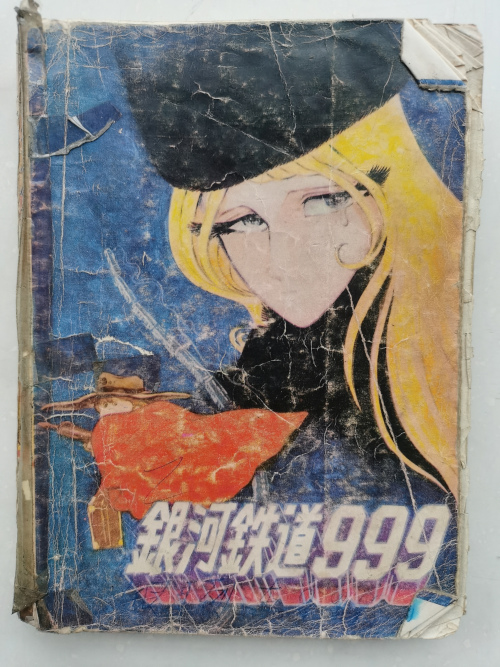
\includegraphics[width=5cm]{pic/银河列车-1.jpg}
      & 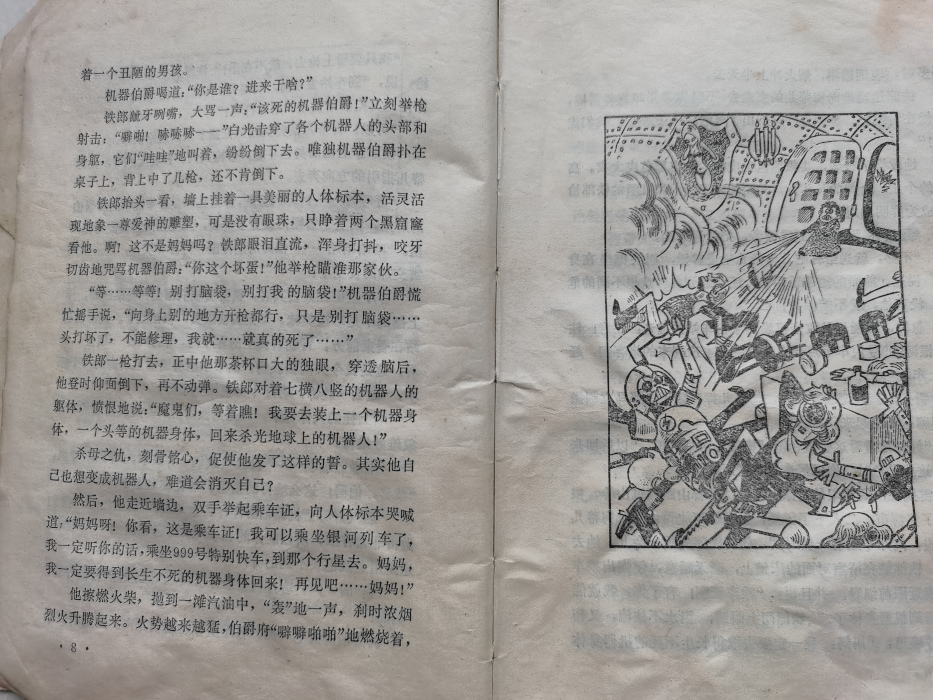
\includegraphics[width=6cm]{pic/银河列车-2.jpg} \\
    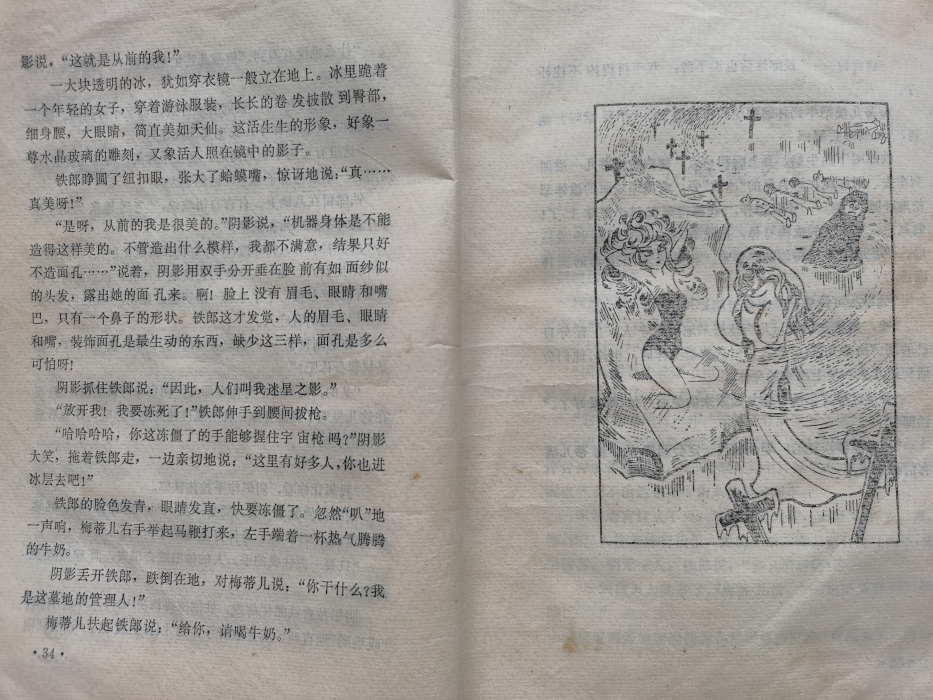
\includegraphics[width=6cm]{pic/银河列车-3.jpg}
      & 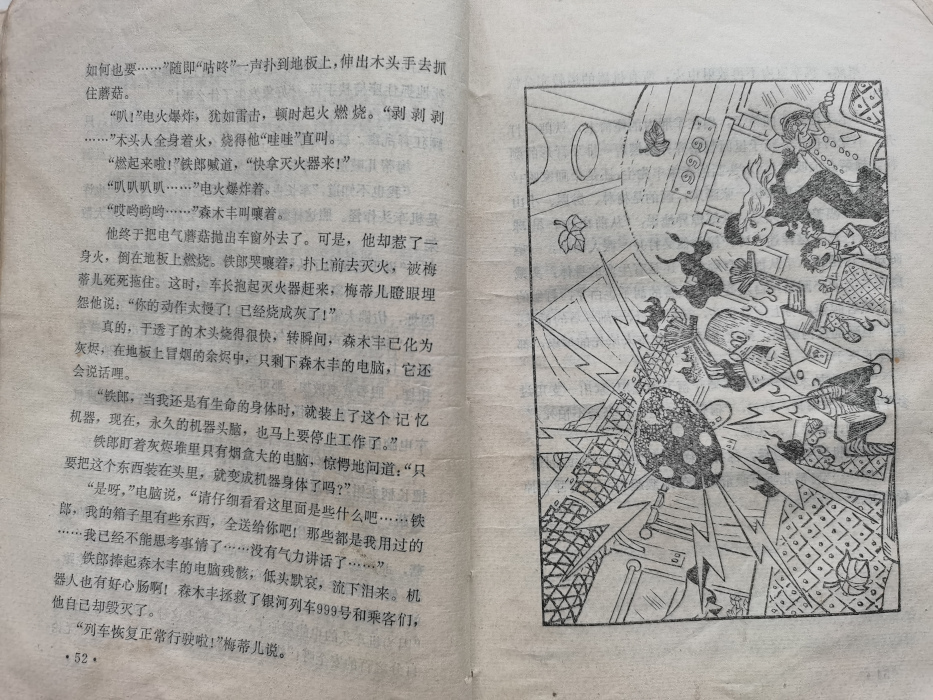
\includegraphics[width=6cm]{pic/银河列车-4.jpg} \\
    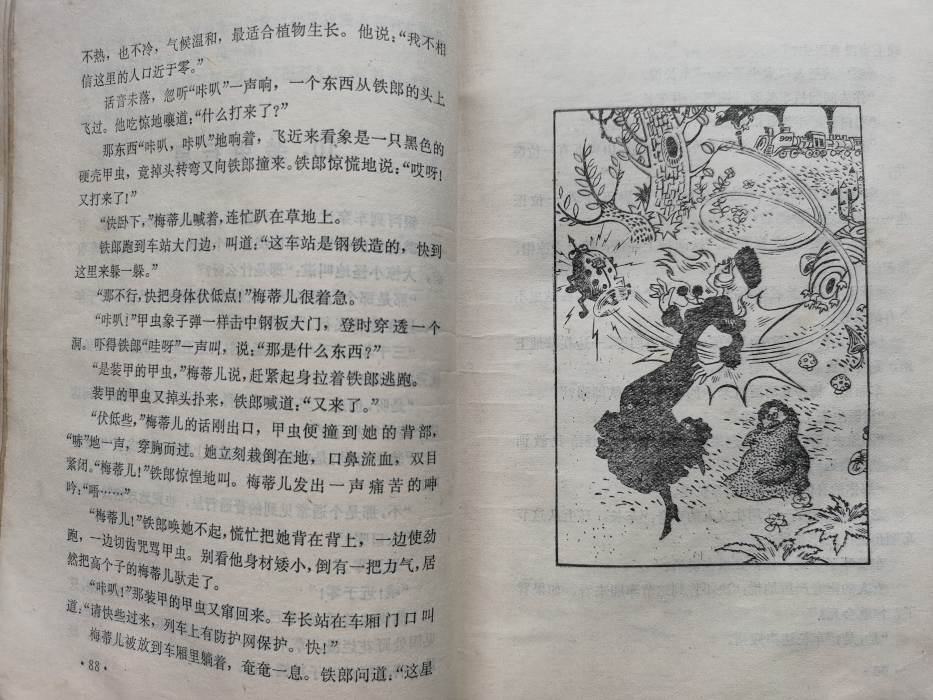
\includegraphics[width=6cm]{pic/银河列车-5.jpg}
      & 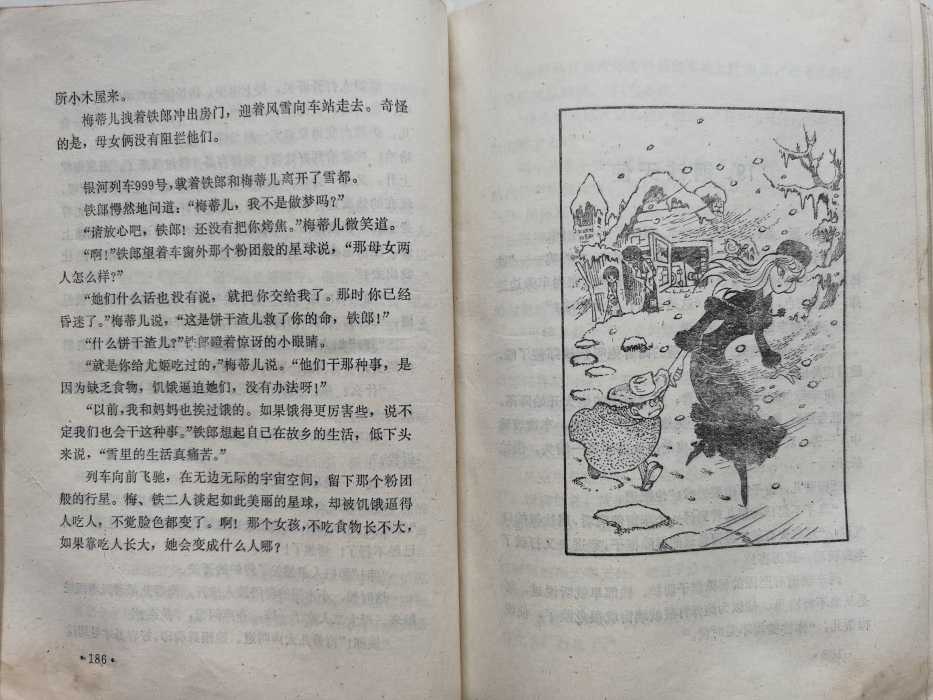
\includegraphics[width=6cm]{pic/银河列车-6.jpg}
  \end{tblr}

  \begin{tblr}{}
    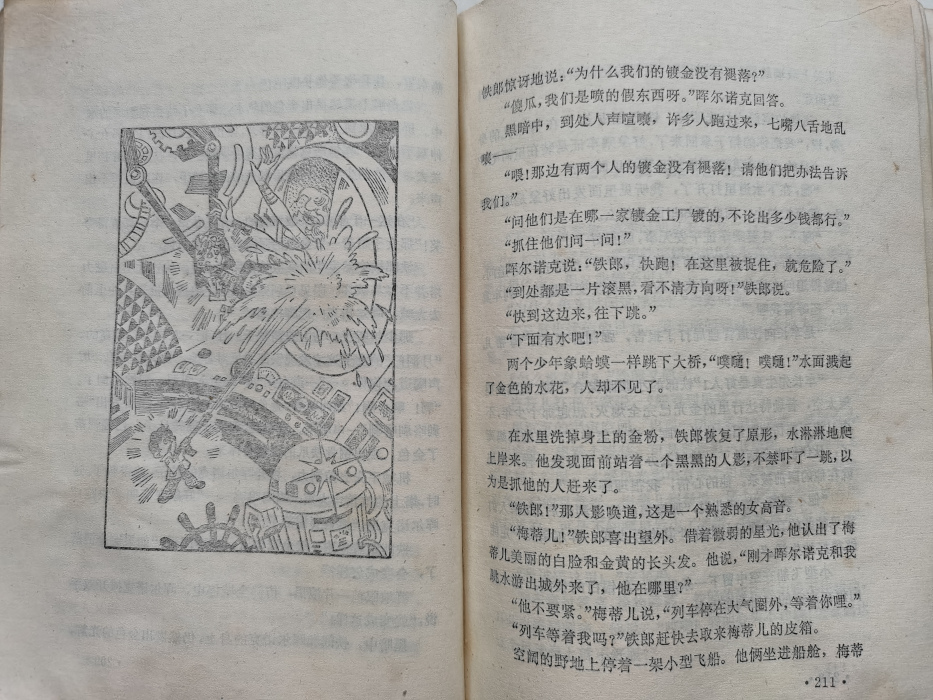
\includegraphics[width=6cm]{pic/银河列车-7.jpg}
      & 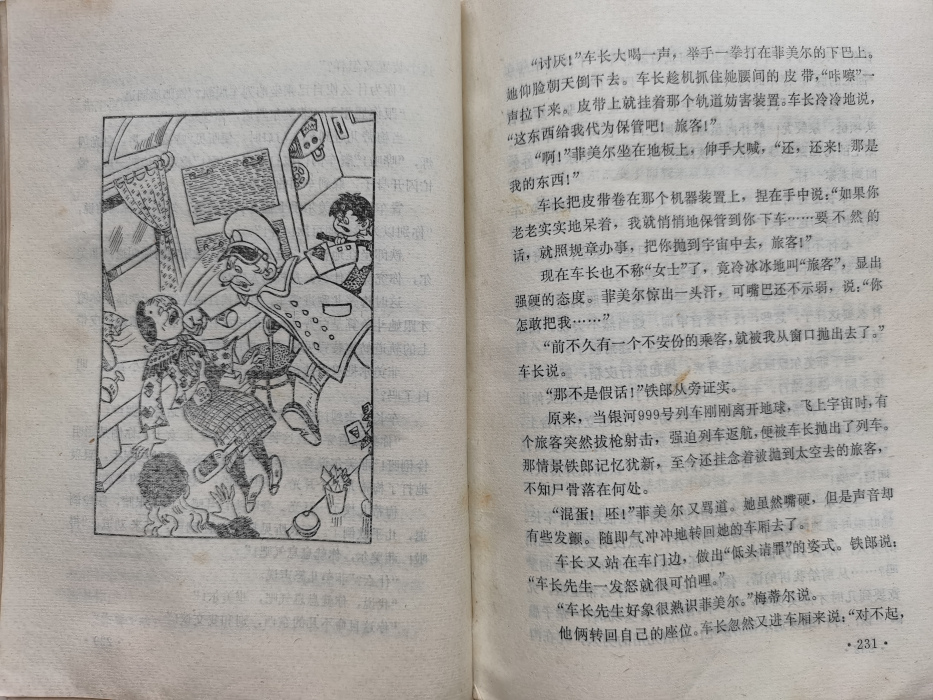
\includegraphics[width=6cm]{pic/银河列车-8.jpg} \\
    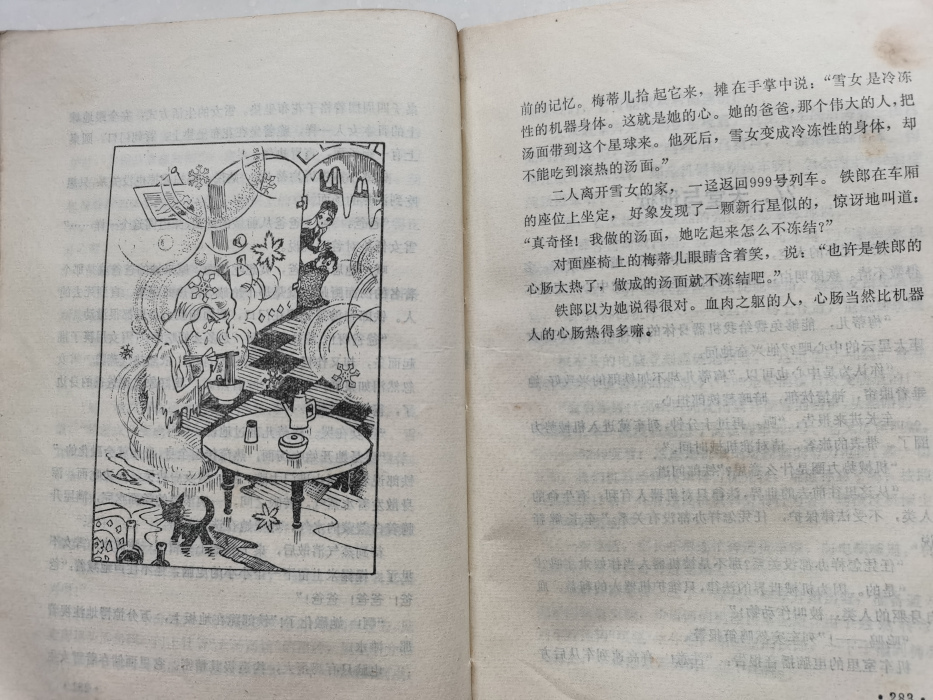
\includegraphics[width=6cm]{pic/银河列车-9.jpg}
    & 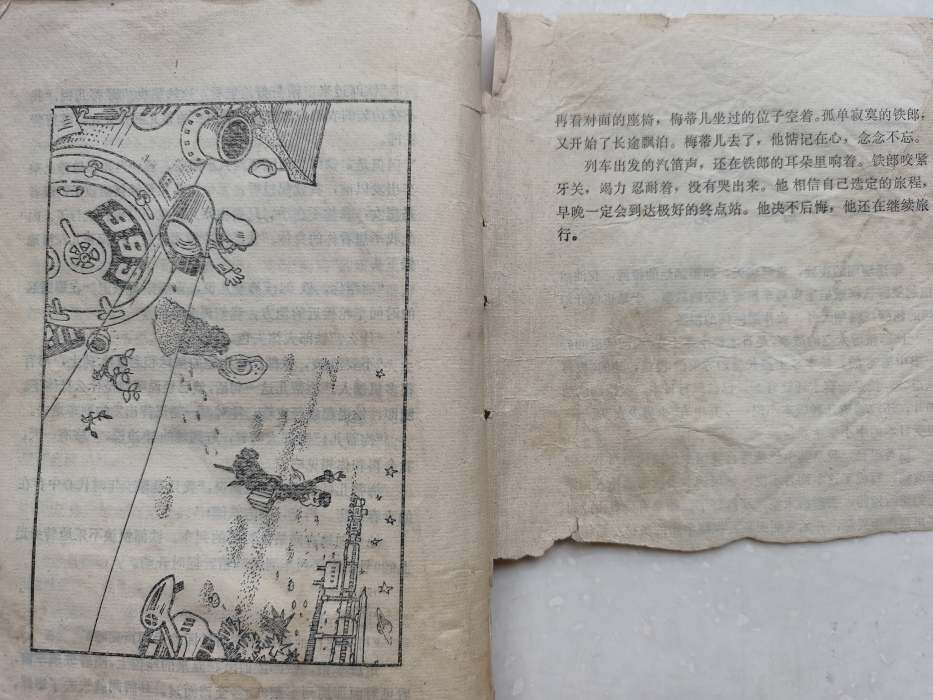
\includegraphics[width=6cm]{pic/银河列车-a.jpg}
  \end{tblr}

\endgroup


\subsection{宝贝二:《圣斗士》}

《\href{https://baike.baidu.com/item/圣斗士/226570}{圣斗士}》和
《\href{https://baike.baidu.com/item/龙珠/545064}{七龙珠}》是初中时期的精神粮食。当然,还有
《\href{https://baike.baidu.com/item/城市猎人/10904}{城市猎人}》、
《\href{https://baike.baidu.com/item/北斗神拳/1014286}{北斗神拳}》。

仅存一本:《女神的胜利卷1 —— 突破!叹息的墙壁》。

\begingroup
  \centering
  \begin{tblr}{}
    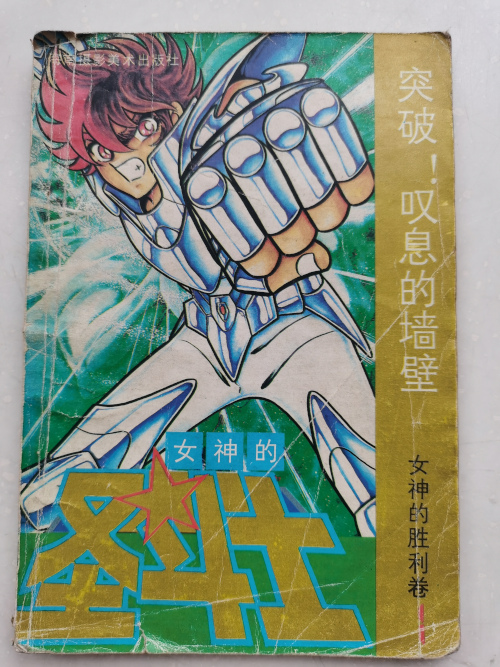
\includegraphics[width=5cm]{pic/圣斗士-1.jpg}
      & 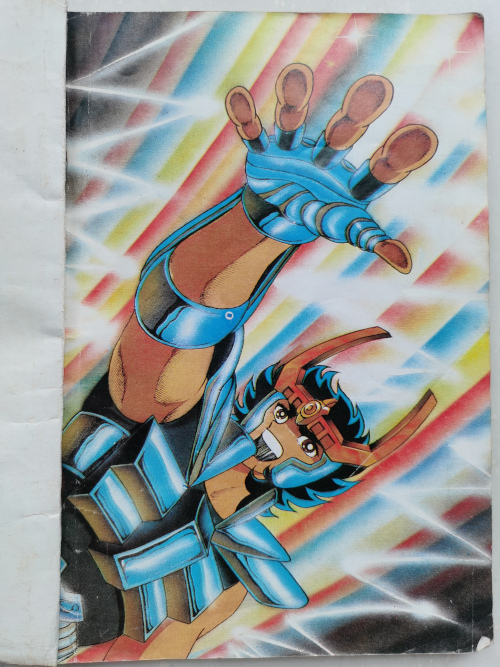
\includegraphics[width=5cm]{pic/圣斗士-2.jpg} \\
    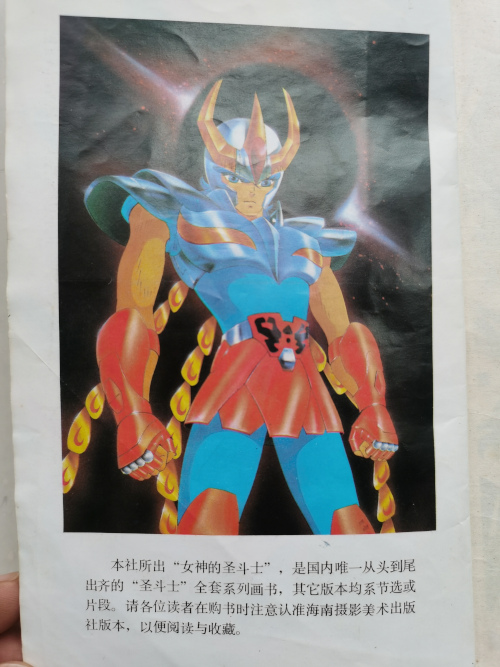
\includegraphics[width=5cm]{pic/圣斗士-3.jpg}
      & 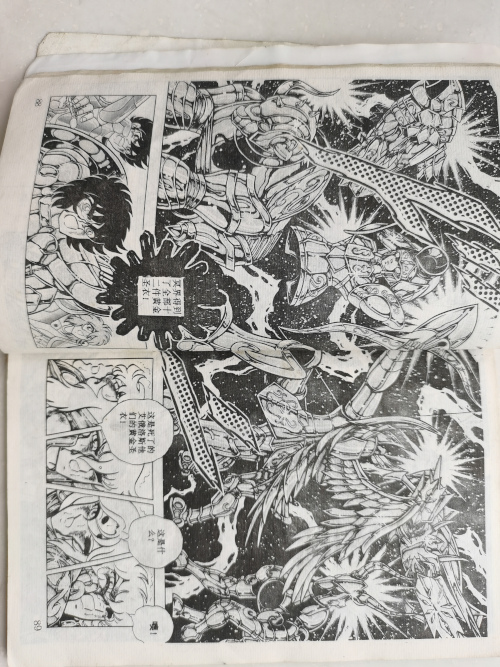
\includegraphics[width=5cm]{pic/圣斗士-4.jpg}
  \end{tblr}

\endgroup


\subsection{宝贝三:军人日记笔记本}

笔记本是我高中期间在一家文具店买的。当时是去文具店买其它的文具,无意中看到这个笔记本。
阅兵式上军人们雄壮的身姿,让我羡慕。我一看就很喜欢,花了重金(好像是十多块钱)将它买下。

笔记本封面内侧,贴着\href{https://baike.baidu.com/item/周慧敏/6702}{周慧敏}的一张海报复印件。
海报是在我同学那里看到的,她的美让我惊为天人,
急忙借来复印一张,贴在笔记本上,每次打开笔记本,就能看见她。

当时手头上有的《七龙珠》的不干胶全都贴在笔记本上了,所以笔记本上彩色很丰富。

\begingroup
  \centering
  \begin{tblr}{}
    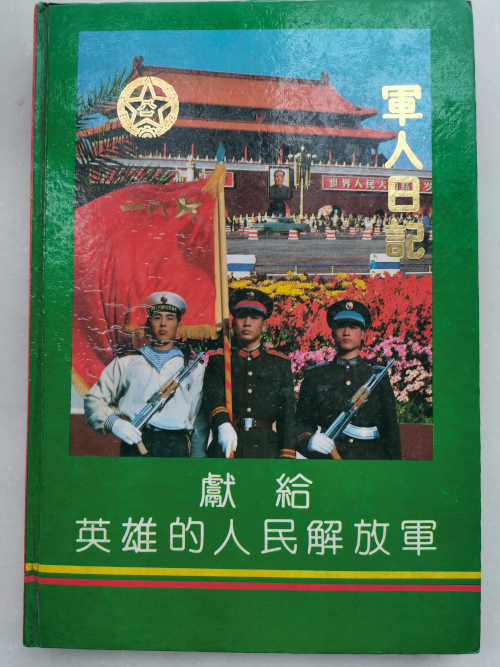
\includegraphics[width=5cm]{pic/军人日记-1.jpg}
      & 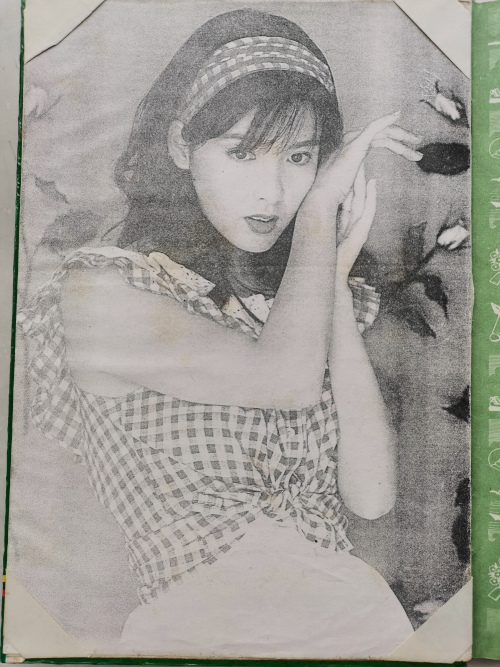
\includegraphics[width=5cm]{pic/军人日记-2.jpg}
      & 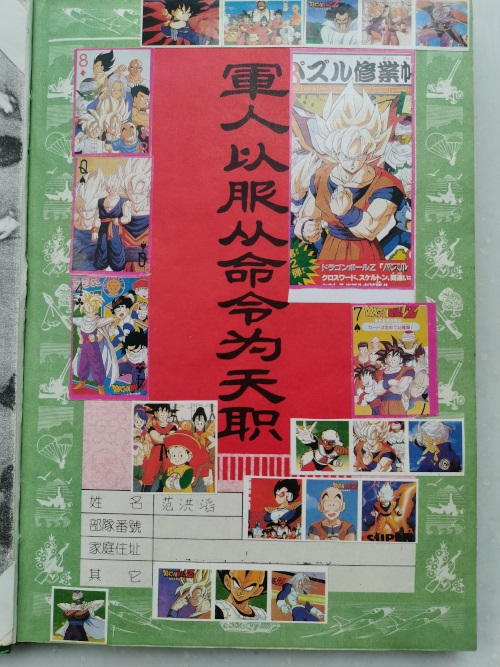
\includegraphics[width=5cm]{pic/军人日记-3.jpg} \\
    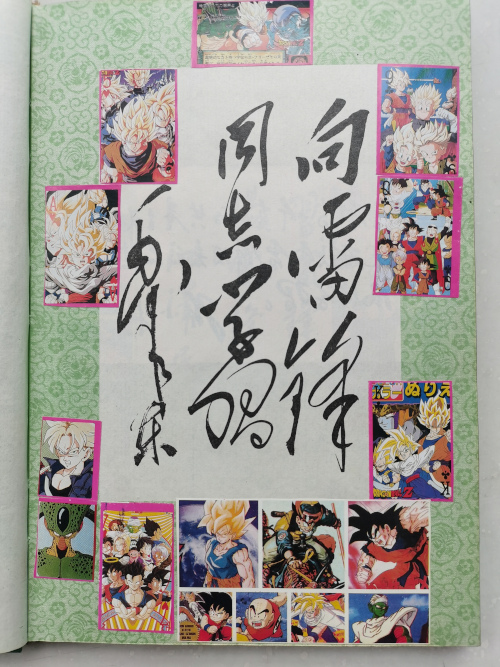
\includegraphics[width=5cm]{pic/军人日记-4.jpg}
      & 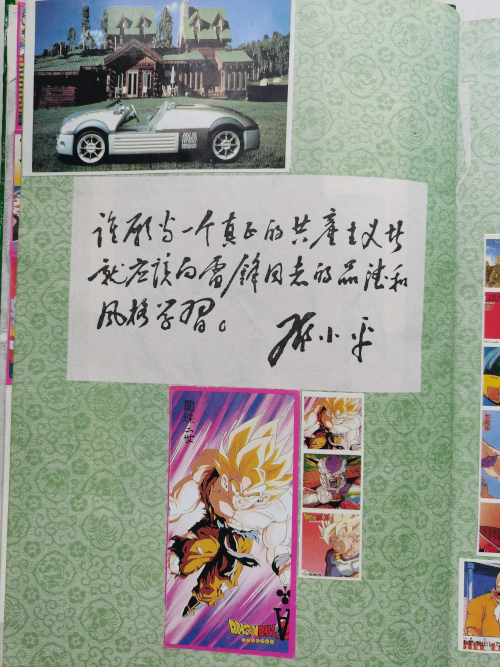
\includegraphics[width=5cm]{pic/军人日记-5.jpg}
      & 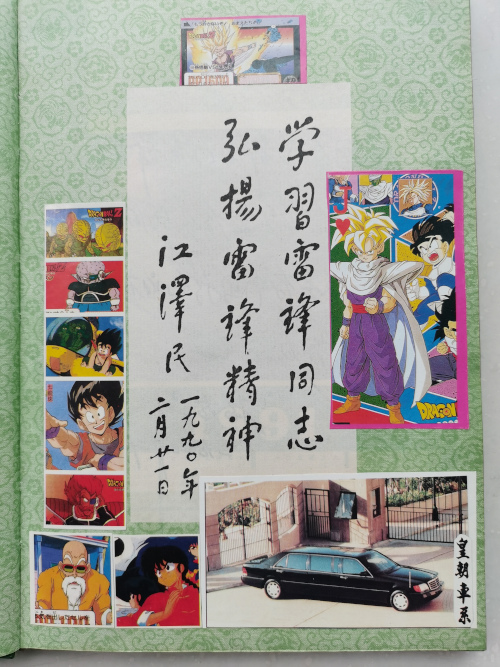
\includegraphics[width=5cm]{pic/军人日记-6.jpg} \\
    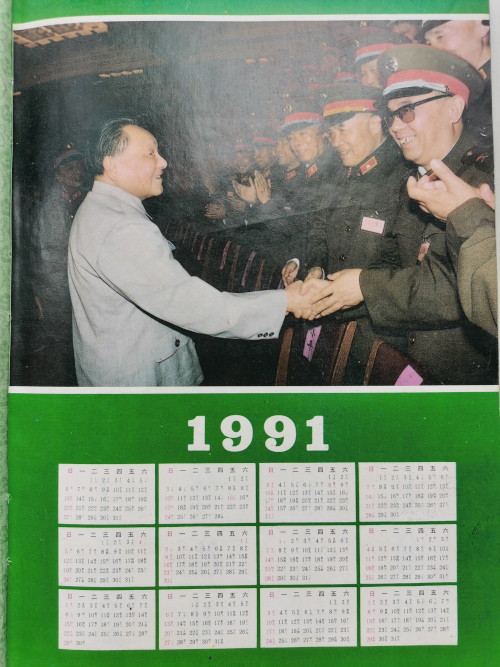
\includegraphics[width=5cm]{pic/军人日记-7.jpg}
      & 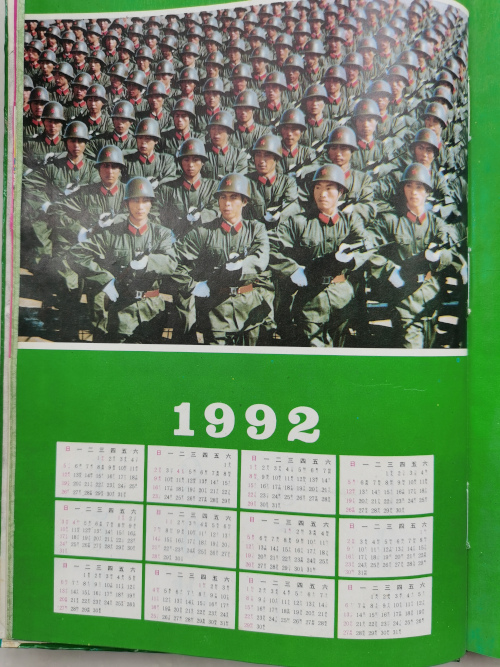
\includegraphics[width=5cm]{pic/军人日记-8.jpg}
      & 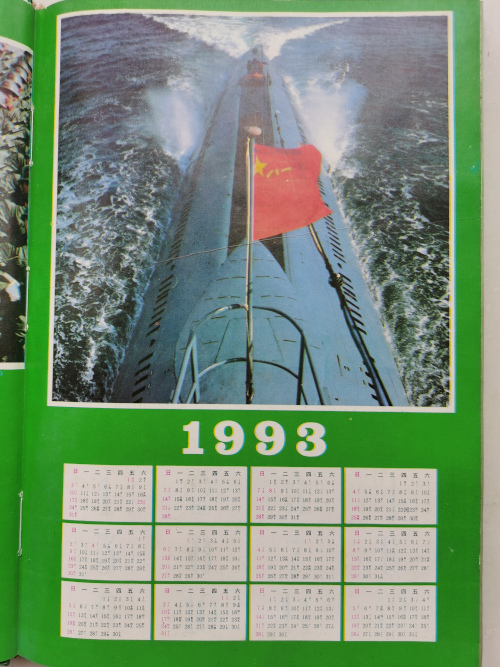
\includegraphics[width=5cm]{pic/军人日记-9.jpg}
  \end{tblr}

  \begin{tblr}{}
    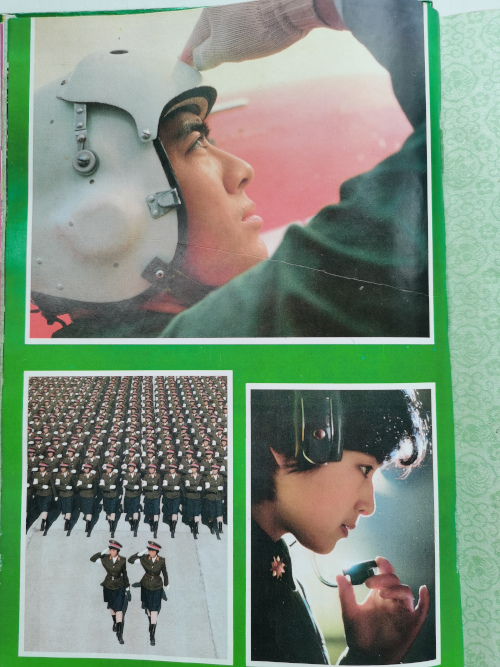
\includegraphics[width=5cm]{pic/军人日记-a.jpg}
      & 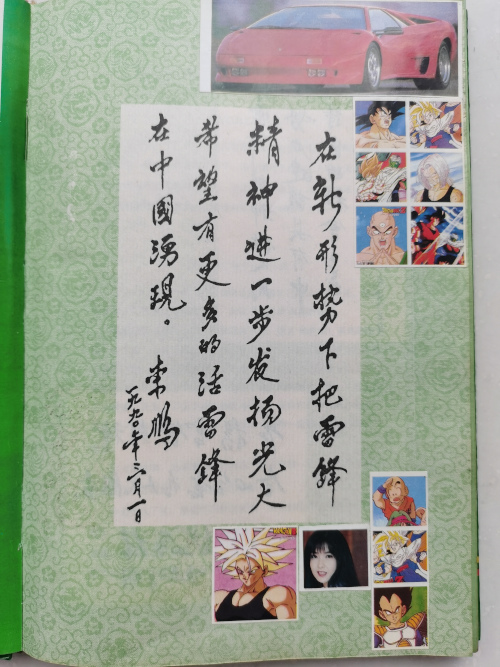
\includegraphics[width=5cm]{pic/军人日记-b.jpg}
      & 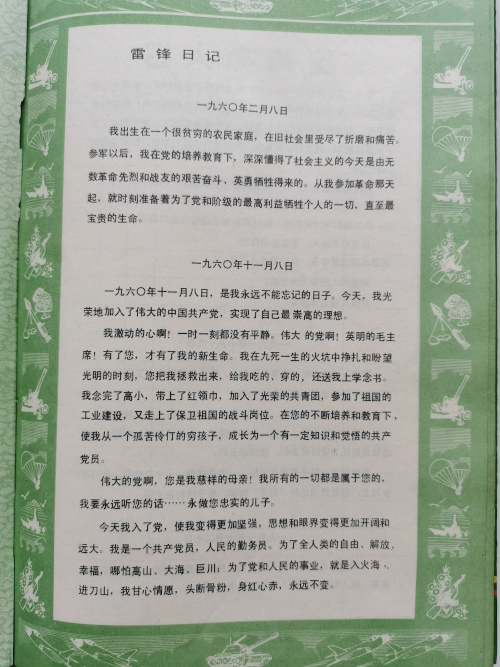
\includegraphics[width=5cm]{pic/军人日记-c.jpg}
  \end{tblr}

\endgroup


\subsection{宝贝四:一张贺卡}

贺卡是大学期间的一位朋友送的。

从小学五六年级开始,就流行在同学之间送贺卡。
这样算下来,直到大学,我送了不少贺卡出去,也收到过不少贺卡。可惜都找不到了。
这张贺卡是因为它正好放在了军人日记的笔记本里,才得以保存下来。

\begingroup
  \centering
  \begin{tblr}{}
    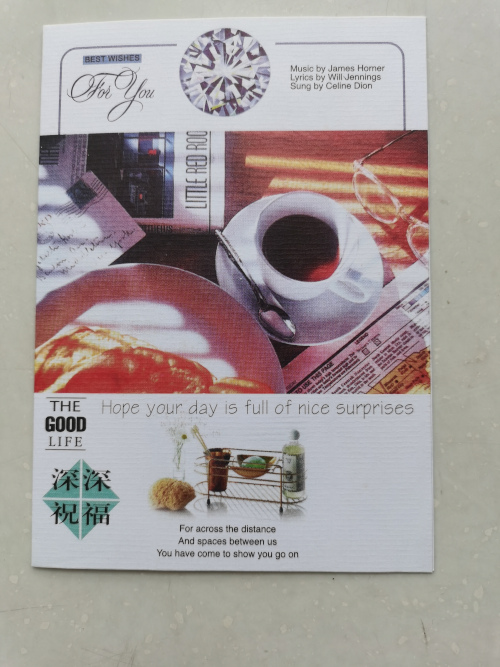
\includegraphics[width=5cm]{pic/贺卡-1.jpg}
      & 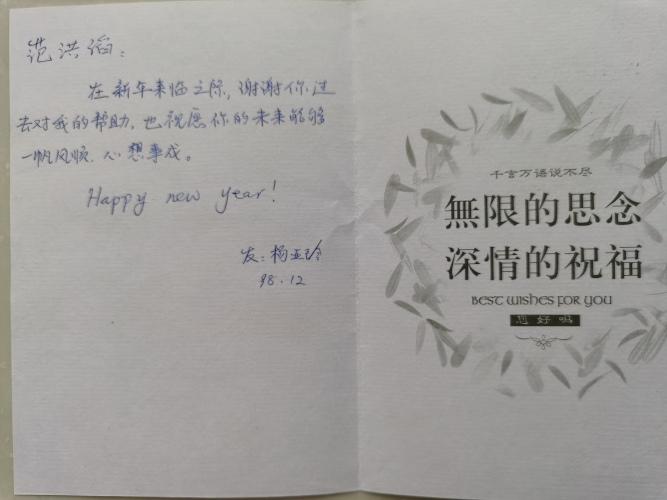
\includegraphics[width=8cm]{pic/贺卡-2.jpg} \\
  \end{tblr}

\endgroup


